\documentclass[11pt]{article}
%\documentclass[dvips,11pt]{article}

% \usepackage{natbib}
% \setlength{\bibsep}{0pt plus 0.3ex}
\usepackage{titlesec}
\titlespacing*{\section}{0pt}{0.3\baselineskip}{0.3\baselineskip}
%,nohead,nofoot
%\usepackage[margin=1n,left=1cm,top=1cm,right=1.75cm,bottom=1.5cm]{geometry}
\usepackage[margin=1in,includeheadfoot,left=1cm,top=0.5cm,right=1.5cm,bottom=0.5cm]{geometry}
%\usepackage[margin=1in,includeheadfoot]{geometry}
\usepackage{url}
\usepackage{cite}
\usepackage{lipsum}
\usepackage{booktabs}
\usepackage{tabularx}
\usepackage{wrapfig}
\usepackage{microtype}
\usepackage{hyperref}
\usepackage{listings}
\usepackage{subfigure}
% ADD THE FOLLOWING COUPLE LINES INTO YOUR PREAMBLE
\let\OLDthebibliography\thebibliography
\renewcommand\thebibliography[1]{
  \OLDthebibliography{#1}
  \setlength{\parskip}{0pt}
  \setlength{\itemsep}{0pt plus 0.3ex}
}

\usepackage[pdftex]{graphicx}
\usepackage{url}
\usepackage{color}
\definecolor{darkred}{rgb}{0.5,0,0}
\definecolor{darkgreen}{rgb}{0,0.5,0}
\definecolor{darkblue}{rgb}{0,0,0.5}
\definecolor{darkaquamarine}{rgb}{0.2,0.4,0.3}
%% macros
\newcommand{\ie}{i.e.}
\newcommand{\eg}{e.g.}
\newcommand{\Fix}[1]{\textbf{[[}{\color{red} #1}\textbf{]]}}
\newcommand{\Mar}[1]{\textbf{[[}{\color{blue} #1}\textbf{]]}}
\newcommand{\MAB}[1]{\textbf{[[}{\color{darkgreen} #1}\textbf{]]}}
\newcommand{\Igor}[1]{\textbf{[[}{\color{darkaquamarine} #1}\textbf{]]}}
\newcommand{\Comment}[1]{}

%% \setlength{\oddsidemargin}{0.25in}
%% \setlength{\textwidth}{6.5in}
%% \setlength{\topmargin}{0in}
%% \setlength{\textheight}{8.5in}

%\renewcommand\Affilfont{\fontsize{9}{10.8}\itshape}
% These force using more of the margins that is the default style

\begin{document}

\title{Finding Bugs in JavaScript Engines with Differential Testing}
\author{}
\date{}

% You can leave out "date" and it will be added automatically for today
% You can change the "\today" date to any text you like

\makeatletter
\def\maketitle{%
  \par{\centering\large\textbf{\@title}\normalsize\par}\vspace{3ex}%
  \par{\@author}%
  \par}
\makeatother

\maketitle

\vspace{-2ex}
\small    
\begin{table}[h!] 
  \centering%% Centro de Inform\'atica - CIn \\
  \begin{tabular*}{.85\linewidth}{l}

    Marcelo d'Amorim and Igor Sim\~oes (M.Sc. student)\\
    
    Postal Address: Av. Jornalista Anibal Fernandes, S/N. Cidade
    Universit\'aria, PE, Brazil, 50.740-560 \\
    
    Email addresses: \{damorim, isol2\}@cin.ufpe.br\\

    Phones: +55 (81) 2126-8430,
    ext. 4379 [work], +55 (81) 98800-2010 [mobile]\\

    Affiliation: Federal University of Pernambuco, Department of
    Computer Science\\

    Contact at Google:~Martin Barbella (mbarbella@google.com)

  \end{tabular*}
\end{table}
\normalsize

\vspace{-2ex}
\begin{abstract}
...
\end{abstract}

\section{Problem Space}

%% Its niche is front-end and
%% back-end web development\Comment{, supported several frameworks and
%%   runtimes (\eg{}, Express.js and Node.js)}.

%% In fact, bugs in JS implementations are often reported by
%% the general public, some of which were reported by our team.
%% (confirmed by engine developers; see
%% Section~\ref{sec:results}) using a prototype of our solution (see
%% Section~\ref{sec:design}).

JavaScript (JS) is one of the most popular programming languages of
today~\cite{business-insider,stackify} largely because of its
widespread use on the web. As common in software, the JS specification
changes regularly\footnote{Recently, the specification went through a
  bigger change compared to prior releases, called by the name of
  ECMAScript6 (ES6)~\cite{es6-features}} to accomodate pressing
demands~\cite{kangax} and these changes often entail sensible changes
in engine implementations that could lead to errors, including
regressions.  Test generation can help reduce the cost of testing, but
the lack of executable specifications is an important obstacle for
finding functional errors.  

%\vspace{-1ex}
\begin{center}
\fbox{
  \begin{minipage}{13.5cm}
    \centering \textit{The goal of this project is to find bugs in
      implementations of JavaScript engines by leveraging diversity
      across implementations.}
  \end{minipage}
}
\end{center}
%\vspace{-1ex}

The novelty of our proposal is the use of multiple engine
implementations (\eg{}, Google's V8, Microsoft's Chakra, etc.) to
assess input validity and to check output
correctness. \emph{Differential testing}\Fix{cite} has been applied in
a variety of contexts\Fix{cite cite}, but it has not been used to find
functional bugs in JS engines \MAB{That's wrong - it has been used at
  least two times: \cite{patra2016learning} and in jsfunfuzz (with a
  smaller scope - most likely regressions)}

\section{Design Space}
\label{sec:design}

\begin{wrapfigure}[13]{r}[0pt]{0.45\textwidth}
\vspace{-5ex}
%\begin{figure}[htbp]
  \centering
  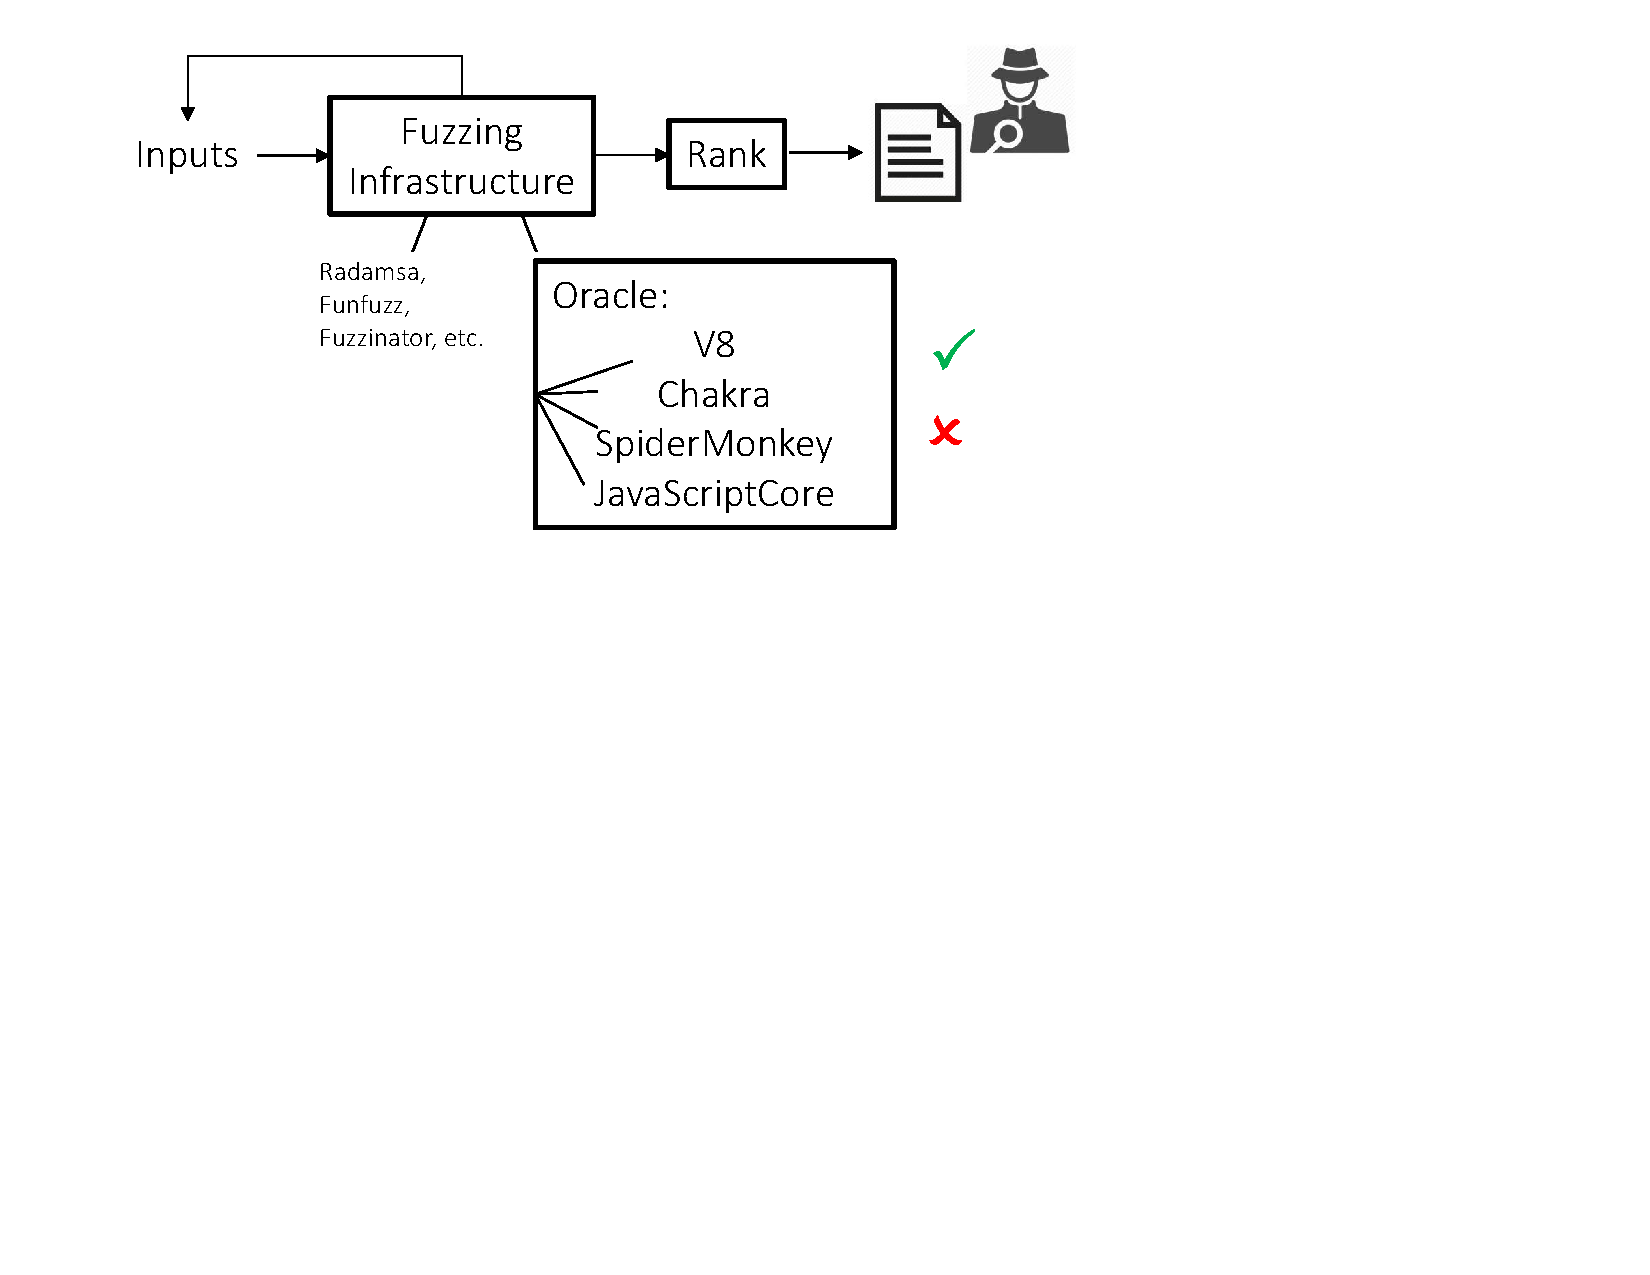
\includegraphics[trim=0 350 200 0,clip,width=0.5\textwidth]{google-awards-workflow}
  \label{fig:workflow}
  \caption{Workflow of Infrastructure.}
%\end{figure}
\end{wrapfigure}
Fuzzing is a popular technique to generate new test inputs from
existing inputs\Fix{cite} with the typical goal of finding
crashes. Several fuzzing methods have been proposed in the past,
varying with respect to how new inputs are generated (\eg{},
mutation-based\Fix{cite}, grammar-based\Fix{cite}, and
random-based\Fix{cite}) and whether or not coverage information is
taken into account in the fuzzing process. Figure~\ref{fig:workflow}
shows a generic pipeline of a fuzzer. JS files are provided as seeded
inputs to bootstrap the process. These files can originate from the
test suites of the engine codebases or from the bug reports in their
issue trackers. \Fix{elaborate}

\section{Related Work}

\Mar{rule of thumb: explain the
  contribution/novelty, then results achieved, and then how it relates
with our proposal.}
\Mar{this is not clear$\rightarrow$}Yang et al. \cite{yang-2011-finding} proposed CSmith\footnote{\url{http://embed.cs.utah.edu/csmith/}}, a grammar-fuzzer 
of C programs to generate invalid entries\Fix{the goal of a
   fuzzer is to generate valid inputs/entries. this is strange}\MAB{the
  goal is to generate valid programs without undefined behavior to
  facilitate differential testing} and
find bugs in several C compilers\Fix{it is strange that you don't mention differential
  testing, which is central in CSmith, and the use of LLVM and GCC as
  oracles.}.\Mar{this is just listing fuzzers. don't do this. try to
  follow rule of thumb above.}Similar fuzzers involving grammar and rules are found in Holler et al. \cite{holler-2012-fuzzing} 
that exposes the LangFuzz to generate entries based in code fragments 
(language grammar, sample code, test suite) and the tool Mozilla 
Funfuzz\footnote{\url{https://github.com/MozillaSecurity/funfuzz}}
that implements a fuzzer based on JavaScript language to improve the 
testing for SpiderMonkey engine, the interpreter of Mozilla Firefox.
\Fix{...}

\MAB{Unfortunately the low-hanging fruit for this project was already
  picked \cite{patra2016learning}, so I believe you should focus on
  taming implementation-specific behavior and/or the testing
  infrastructure (i.e. how to organize all those fuzzers and make them
  work together). You might also want to mention the possibility of
  fuzzing
  \href{https://developer.mozilla.org/en-US/docs/WebAssembly}{WebAssembly}
  directly: LLVM already has (some) support for targeting WebAssembly,
  which means that we'll be able to run, in the near future, pretty
  much every language with an LLVM-backed compiler in a browser.}

\section{Current Results}
\label{sec:results}

\Igor{
  Nowadays, we used six javascript engines suites with approximately 2K of javascript files 
  that could be fuzzed. Currently, using our infrastructure we reported \Fix{13}
  bugs so far. The Table~\ref{tab:bugs} exposes all bugs found and reported by our team.
  At this moment, the status are: \Fix{6} issues was tagged as new, \Fix{4} was confirmed
  and \Fix{2} of them was merged and closed. Unfortunally, \Fix{1} of them was rejected
  due the engine does not follows the specification and dozens of others warnings already been
  reported previously.

  The Figure~\ref{fig:bug-chakra} exposes a fuzzed file generated by radamsa in our environment, it was observed
  that the fuzzer replace the empty string at Line 3 and replace it with the hexadecimal value "\textbackslash x00".
  The bug manifests in Line 7, according to ES6 specification on Mozilla dev website
  \footnote{Unary Plus \url{https://developer.mozilla.org/en-US/docs/Web/JavaScript/Reference/Operators/Arithmetic_Operators}},
  the unary plus converts the variable to an integer if it is a valid value
  otherwise returns NaN. The Figure~\ref{fig:pattern} shows the log output from our infrastructure,
  see that we set automatically this testcase as high priority because it is a failure by assertion.
  The differential test across all engines, shows a unexpected behaviour of ChakraCore engine that passes in this test case.
  It was necessary a manual inspection to check if it is a real bug, we observed that 
  ChakraCore indentify "\textbackslash x00" as a null terminator instead of invalid parser object making
  the unary plus converts null to 0.
}
\Fix{nao estou conseguindo mesclar dois listings com subfigure, por favor alguem tenta fazer isso por mim.}
\Igor{Coloco outro caso de bug reportado?}

\lstdefinelanguage{JavaScript}{
  keywords={break, case, catch, continue, debugger, default, delete, do, else, finally, for, function, if, in, instanceof, new, return, switch, this, throw, try, typeof, var, void, while, with},
  morecomment=[l]{//},
  morecomment=[s]{/*}{*/},
  morestring=[b]',
  morestring=[b]",
  sensitive=true
}

\begin{figure}[htbp]
    \centering
    \begin{subfigure}[b]{0.4}
        \centering
        \scriptsize
        \lstset{
            language=JavaScript,
            keywords={function, return},
            escapeinside={@}{@},
            numbers=left,xleftmargin=1em,frame=single,framexleftmargin=0.5em,
            basicstyle=\ttfamily\scriptsize, boxpos=c,
            numberstyle=\tiny,
            linewidth=6cm
        }
\begin{lstlisting} 
var a = {
    valueOf: function () {
-    return ""
+    return "\x00"
    }
}
assert(+a === 0)
\end{lstlisting}
        \normalsize
        \caption{
            \label{fig:bug-chakra}Fuzzed file shows an unexpected behaviour on ChakraCore
        }        
    \end{subfigure}
    \begin{subfigure}[b]{0.4}
\begin{lstlisting}[basicstyle=\ttfamily]
Priority: HIGH
Pattern:
-----JavaScriptCore
Error: Test failed
-----Chakra
-----SpiderMonkey
Error: Test failed
-----v8
Error: Test failed
\end{lstlisting}
\caption{\label{fig:pattern}\Fix{JSFuzz} output log}
\end{subfigure}
\end{figure}
  

\begin{table}[]
    \centering
    \caption{Bugs found and reported by \Fix{JSFuzz} team}
    \label{tab:bugs}
    \begin{tabular}{|c|c|c|c|}
    \hline
    Issue    & Engine                                                          & Status                                                                            & \multicolumn{1}{c|}{Url}                                                                                                                      \\ \hline
    Bug \#1  & Chakra                                                          & Fixed                                                                             & \href{https://github.com/Microsoft/ChakraCore/issues/4978}{\#4978}                                                                                           \\ \hline
    Bug \#2  & Chakra                                                          & Rejected                                                                          & \href{https://github.com/Microsoft/ChakraCore/issues/4979}{\#4979}                                                                              \\ \hline
    Bug \#3  & JavascriptCore                                                  & New                                                                               & \href{https://bugs.webkit.org/show\_bug.cgi?id=184629}{\#184629}                                                                                               \\ \hline
    Bug \#4  & JavascriptCore                                                  & New                                                                               & \href{https://bugs.webkit.org/show\_bug.cgi?id=184749}{\#184749}                                                                                               \\ \hline
    Bug \#5  & Chakra                                                          & Confirmed                                                                         & \href{https://github.com/Microsoft/ChakraCore/issues/5033}{\#5033}                                                                                           \\ \hline
    Bug \#6  & Chakra                                                          & Fixed                                                                             & \href{https://github.com/Microsoft/ChakraCore/issues/5038}{\#5038}                                                                                           \\ \hline
    Bug \#7  & Chakra                                                          & Confirmed                                                                         & \href{https://github.com/Microsoft/ChakraCore/issues/5065}{\#5065}                                                                                           \\ \hline
    Bug \#8  & \begin{tabular}[c]{@{}c@{}}Chakra\\ JavascriptCore\end{tabular} & \begin{tabular}[c]{@{}c@{}}Confirmed (Chakra)\\ New (JavascriptCore)\end{tabular} & \begin{tabular}[c]{@{}l@{}}\href{https://github.com/Microsoft/ChakraCore/issues/5067}{\#5067}\\ \href{https://bugs.webkit.org/show\_bug.cgi?id=185130}{\#185130}\end{tabular} \\ \hline
    Bug \#9  & JavascriptCore                                                  & New                                                                               & \href{https://bugs.webkit.org/show\_bug.cgi?id=185127}{\#185127}                                                                                               \\ \hline
    Bug \#10 & \begin{tabular}[c]{@{}c@{}}Chakra\\ JavascriptCore\end{tabular} & \begin{tabular}[c]{@{}c@{}}Confirmed (Chakra)\\ New (JavascriptCore)\end{tabular} & \begin{tabular}[c]{@{}l@{}}\href{https://github.com/Microsoft/ChakraCore/issues/5076}{\#5076}\\ \href{https://bugs.webkit.org/show\_bug.cgi?id=185156}{\#185156}\end{tabular} \\ \hline
    Bug \#11 & JavascriptCore                                                  & New                                                                               & \href{https://bugs.webkit.org/show\_bug.cgi?id=185197}{\#185197}                                                                                               \\ \hline
    Bug \#12 & JavascriptCore                                                  & New                                                                               & \href{https://bugs.webkit.org/show\_bug.cgi?id=185208}{\#185208}                                                                                               \\ \hline
    Bug \#13 & Chakra                                                          & New                                                                               & \href{https://github.com/Microsoft/ChakraCore/issues/5128}{\#5128}                                                                      \\ \hline
    \end{tabular}
    \end{table}

\section{Data Policy}

The results produced with this research will be made available to the
public and to the research community.  All tools and data sets
developed will be available online, and the software will be released
under an open source license.


\footnotesize
\bibliographystyle{plain}
\bibliography{tmp}

\end{document}

